\documentclass[12pt]{utscapstone}
\usepackage[left=40mm, right=25mm, top=30mm, bottom=30mm, twoside]{geometry} 
\geometry{a4paper}                   % ... or a4paper or a5paper or ... 
\renewcommand{\baselinestretch}{1.5}

%\geometry{landscape}                % Activate for for rotated page geometry
%\usepackage[parfill]{parskip}    % Activate to begin paragraphs with an empty line rather than an indent

\usepackage{graphicx}
\usepackage{lscape}
\usepackage{amssymb}
\usepackage{epstopdf}
\usepackage{algorithm}
\usepackage{algorithmic}
\usepackage{subfig}
\usepackage{float}
\usepackage{wrapfig}
\usepackage{fancyhdr}
\usepackage{natbib}
\captionsetup{margin=10pt,font=small,labelfont=bf}
\usepackage[raggedright]{titlesec}
\usepackage{amsmath}
%\usepackage{subfigure} %subfigure for multiple figures

\bibpunct{(}{)}{;}{a}{,}{,}
\renewcommand{\cite}\citep


\pagestyle{fancyplain}


\fancyhead[LO,LE]{\small\textit{Learning Repetitive Gestures By Demonstration Using Nonlinear Oscillators}}
\fancyhead[RO,RE]{}
\fancyfoot[LO,RE]{}
\fancyfoot[RO,LE]{\thepage}
\fancyfoot[C]{}

\renewcommand{\headrulewidth}{0.4pt}
\renewcommand{\footrulewidth}{0.4pt}
\renewcommand{\plainheadrulewidth}{0.4pt}
\renewcommand{\plainfootrulewidth}{0.4pt}
\newcommand{\HRule}{\rule{\linewidth}{0.5mm}}

\DeclareGraphicsRule{.tif}{png}{.png}{`convert #1 `dirname #1`/`basename #1 .tif`.png}

\begin{document}
\pagenumbering{roman}

\begin{titlepage}

\begin{center}
University of Technology, Sydney

Faculty of Engineering and Information Technology\\[1.0cm]

{  \bfseries Learning Repetitive Gestures By Demonstration Using Nonlinear Oscillators}\\[0.5cm]


\textbf{William bond}\\[1.0cm]

Student Number: 10555163

Project Number: S11-006

Major: Mechanical and Mechatronic Engineering\\[0.5cm]

Supervisor: Dr Alen Alempijevic\\[1.0cm]


\includegraphics[width=0.5\textwidth]{figures/ralogo}\\


\includegraphics[width=0.4\textwidth]{figures/caslogo}\hspace{20mm}

\includegraphics[width=0.4\textwidth]{figures/utslogo}\\[1cm]

A 12 Credit Point Project submitted in partial fulfilment of the requirement for the Degree of Bachelor of Engineering\\[1.5cm]

20th June, 2012

\end{center}

\end{titlepage}

\chapter*{Statement of Originality}
I declare that I am the sole author of this report, that I have not used fragments of text from other sources without proper acknowledgment, that theories, results and designs of others that I have incorporated into my report have been appropriately referenced and all sources of assistance have been acknowledged.

\chapter*{Abstract}
{  \bfseries Shape Based Recognition and Fast Learning Techniques For Autonomous Robots }
William Bond, S11-006.\\


My Abstract WILL be written here... maybe.

\chapter*{Acknowledgements}

I would like to thank my supervisor XXXX for his help and guidance throughout this whole project, he has been a tremendous help towards making this thesis possible. Special thanks also to XXX for lending their experience and knowledge, and helping me out when I needed third party input.
I would especially like to thank my family for their enending support in my academic progression.

The work represented in this project is supported by the ARC Centre of Excellence programme, the University of Technology and the RobotAssist development project.


\tableofcontents

\listoffigures

\chapter*{Nomenclature}

\begin{center}
  \begin{tabular}{| c | l |}\hline
    \textbf{Term} & \textbf{Definition}\\ \hline
    HRI & Human-robot interaction\\
    RGB & Red Green Blue\\
    3D & Three dimensional\\
    DOF & Degree Of Freedom\\
    GUI & Graphical User Interface\\
    RPY & Roll, Pitch and Yaw\\
    PCL & Point Cloud Library\\
    RA & RobotAssist\\
    \hline
  \end{tabular}
\end{center}

\clearpage
\pagenumbering{arabic}

\chapter{textools}
\section{uasable tools}
Citing something
Here I will cite something - Nehaniv et al \cite{nehaniv2005} 

Dot Points
\begin{itemize} 
	\item Dot point
	\item etc
	\item etc 
\end{itemize} 

Italics (emphasis)
\emph{Here the text will be in italics, then will cite something} \cite{chawala}.

Referring to other sections of the report.
Referring to something in a section like \ref{scope}.
Anything with a label can be referred to again later as in Fig \ref{fig:rgbanddepth}. 

Image insertion
\begin{figure}[h]
\centering
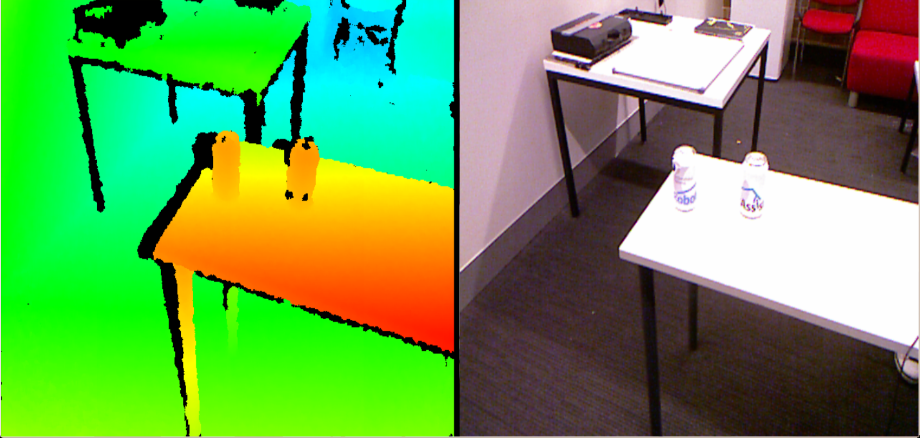
\includegraphics[width=0.75\textwidth]{figures/rgbanddepth}
\caption[This goes into the contents.]{Image insertation is annoying, it puts the image onto the start of the new page only. This could probably be fixed though...}
\label{fig:rgbanddepth}
\end{figure}

Table insertation
\begin{table}[ht]
\begin{centering}
\begin{tabular}{|c|c|c|}
\hline
 & SwissRanger 4000 & Kinect\\
 \hline
 Range (m) & 10 & 3\\
 \hline
 Frame Rate (Hz) & 50 & 30\\
 \hline
 Output Resolution (Pixels) & 176x144 & 640x480\\
 \hline
 Precision (mm) & 10 & 1.3\\
 \hline 
\end{tabular}
\caption{Comparison of SwissRanger and Kinect camareas}
\label{sensorcomparison}
\end{centering}
\end{table}

Equation insertation
\begin{align}
\ddot{x} + \epsilon(x^2 - 1)\dot{x} + x = 0
\end{align}
\begin{align}
\dot{x} &=  \alpha(\mu-(x^2+y^2))x - \omega y \label{eqn:hopf1}\\
\dot{y} &=  \alpha(\mu-(x^2 + y^2))y + \omega x \label{eqn:hopf2}\\
\dot{\omega} &= -\epsilon F(t)\frac{y}{\sqrt{x^2+y^2}} 
\end{align}
\begin{align}
\dot{r} &= \alpha(\mu-r^2)r\\
\dot{\phi} &= \omega
\end{align}

Here is an UNREFERENCED MATRIX.
 \[\left( \begin{array}{ccccc}
n & \theta_{n+1} & d_{n+1} & a_{n+1} & \alpha_{n+1}\\
0 & \theta_{1} & 0 & 0 & 90\\
1 & \theta_{2} & -175 & 400 & 0\\
2 & \theta_{3} & 75 & 0 & 90\\
3 & \theta_{4} & 330 & 0 & 90\\
4 & \theta_{5} & 0 & 0 & -90\\
5 & \theta_{6} & 0 & 0 & 0 \end{array} \right) \Rightarrow \left( \begin{array}{cccc}
c\theta_{n+1} & -s\theta_{n+1}c\alpha_{n+1} & s\theta_{n+1}s\alpha_{n+1} & a_{n+1}c\theta_{n+1}\\
s\theta_{n+1} & c\theta_{n+1}c\alpha_{n+1} & -c\theta_{n+1}s\alpha_{n+1}  & a_{n+1}s\theta_{n+1}\\
0 & s\alpha_{n+1} & c\alpha_{n+1} & d_{n+1}\\
0 & 0 & 0 & 1\end{array}\right)\]
\\

Referring to an equation
refer like this - \ref{eqn:hopf1}.

Symbols inserted into a sentance like this $\epsilon$. And \(x = r \cos(\phi)\) and \(y = r \sin(\phi)\).

\pagebreak
PAGEBREAK

LANDSCAPE MODE ON NEXT PAGE!
\begin{landscape}
\centering
\vspace{10mm}
\small
\[ \left( \begin{array}{cccc}
c_{1}& 0&  s_{1}& 0\\
 s_{1}& 0& -c_{1}& 0\\
       0& 1&        0& 0\\
       0& 0&        0& 1
\end{array}\right) \times \left( \begin{array}{cccc}
 c_{2}& -s_{2}& 0& 400c_{2}\\
 s_{2}&  c_{2}& 0& 400s_{2}\\
       0&        0& 1&        -175\\
       0&        0& 0&           1
\end{array}\right) \times \left( \begin{array}{cccc}
 c_{3}& 0&  s_{3}&  0\\
 s_{3}& 0& -c_{3}&  0\\
       0& 1&        0& 75\\
       0& 0&        0&  1
\end{array}\right) \times \left( \begin{array}{cccc}
 c_{4}& 0&  s_{4}&   0\\
 s_{4}& 0& -c_{4}&   0\\
       0& 1&        0& 330\\
       0& 0&        0&   1
\end{array}\right) \times \left( \begin{array}{cccc}
 c_{5}&  0& -s_{5}& 0\\
 s_{5}&  0&  c_{5}& 0\\
       0& -1&        0& 0\\
       0&  0&        0& 1
\end{array}\right) \times \left( \begin{array}{cccc}
 c_{6}& -s_{6}& 0& 0\\
 s_{6}&  c_{6}& 0& 0\\
       0&        0& 1& 0\\
       0&        0& 0& 1
\end{array}\right)\]\\
\vspace{10mm}
\normalsize$=\ $\\
\footnotesize
\[ \left( \begin{array}{cccc}
s_{6}(A) + c_{6}(B)
&c_{6}(A) - s_{6}(B)
&c_{5}(c_{12}s_{3} + c_{13}s_{2}) - s_{5}(G)
&400c_{12} - 100s_{1} + 330c_{12}s_{3} + 330c_{13}s_{2}\\

- s_{6}(c_{14} - s_{4}(C)) - c_{6}(c_{5}(EC) - s_{5}(D)
&s_{6}(c_{5}(EC) - s_{5}(D)) - c_{6}(c_{14} - s_{4}(C))
&s_{5}(EC) + c_{5}(D)
&100c_{1} + 400c_{2}s_{1} + 330c_{2}s_{13} + 330c_{3}s_{12}\\

- c_{6}(F) - s_{46}(c_{2}s_{3} + c_{3}s_{2})
&s_{6}(F) - c_{6}s_{4}(c_{2}s_{3} + c_{3}s_{2})
&- c_{5}(c_{2+3}) - c_{4}s_{5}(s_{2+3})
&400s_{2} - 330c_{23} + 330s_{23}\\

0&0&0&1
\end{array}\right)\]
\normalsize
Landscape mode will end in 3...2...1..
\end{landscape}

Compounded images.
\begin{figure}[ht]
\centering
\subfloat[1st figure]{\label{fig:example1}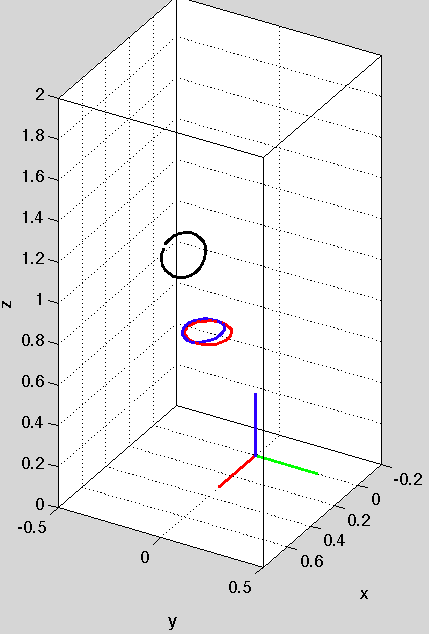
\includegraphics[scale=0.3]{figures/middleangle}}\\
\vspace{2mm}
\subfloat[2nd figure]{\label{fig:example2}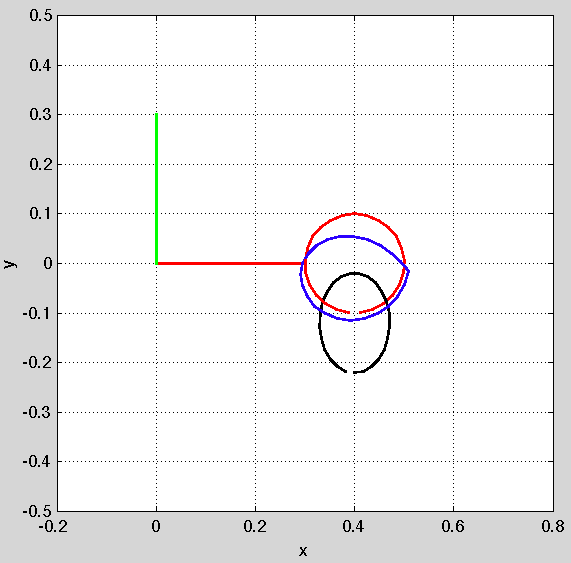
\includegraphics[scale=0.2]{figures/middleXY}}\hspace{5mm}
\subfloat[3rd fig]{\label{fig:example3}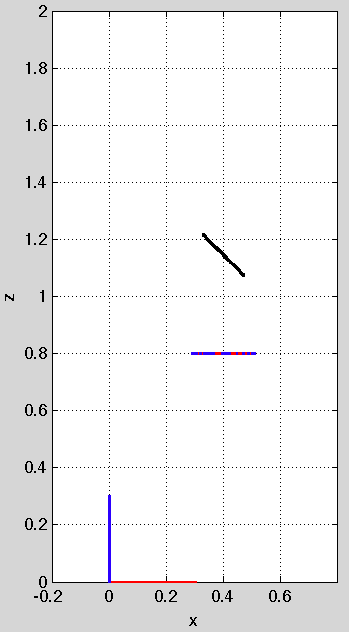
\includegraphics[scale=0.3]{figures/middleXZ}}\hspace{5mm}
\subfloat[4th fig]{\label{fig:example4}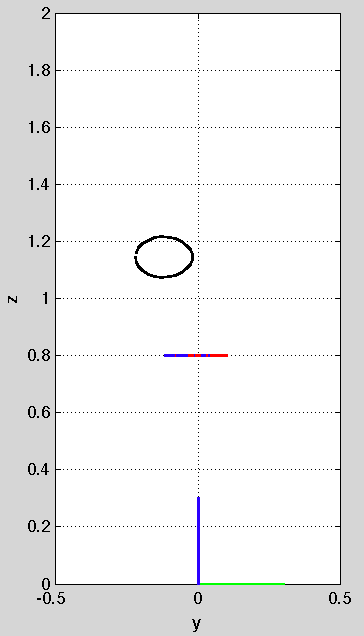
\includegraphics[scale=0.3]{figures/middleYZ}}
\caption[This will appear in the table of contents]{Explain your picture with a quick and simple explanation}
\label{fig:middle}
\end{figure}


Let's try two side by side with Fig.\ref{fig:example1} or Fig.\ref{fig:example2} or I can just refer to Fig.\ref{fig:middle}

I'll also talk later in Sec.\ref{sec:objectseparating} on Object Separating.

%Make a code comment like this. Awesome huh.

\chapter{Introduction}
\label{intro}
\section{The Development and need for Autonomous Robots in the Home}
\label{needforrobotsathome}

\section{The Development of a Robust and Efficient method of Object Detection}
\label{needfordetection}


\section{The Robotic Recognition Problem}
\label{recognitionproblem}


\section{Proposed Method Validation Using The RobotAssist Platform}
\label{methodvalidation}

\section{Relevent Publications To This Capstone}
\label{releventpublications}

\section{Capstone Project Report Guideline}
\label{projectguide}

\section{Scope}
\label{scope}

\chapter{Literature Review}
\label{litreview}

\section{Getting a Physical 3D Space into a Computer}
\label{3d3computer}


\section{Separation of Object of Interest}
\label{sec:objectseparating}


\subsection{A SUBSECTION - HOW AWESOME!}

\subsection{Subsections don't NEED a label}


\section{Recognition and Learning}
\label{randl}

\subsection{Exportation of Usable Data}

\subsection{Sub2}
\label{sec:sub2label}

\section{Recommendations}
\label{sec:recommendations}

\chapter{Object Recognition and Primitive Feature Classification}
\label{recogniseclassify}

\section{How does my code collect point clouds}
\label{pccollection}

\section{How does my code recognise object from a blank point cloud}
\label{objectrecognise}

\section{How does my code find the basic classification of an object based on primitive features}
\label{classification}


\chapter{Fast Object Learning and Associative matching}
\label{fastlearningmatching}

\section{How does my code store object specific features}
\label{featurestoring}

\section{How does my code create associations between previously collected specific features, in the effort to recognise a previously found object.}
\label{associatedfeatures}

\section{How does my code associate similar matches of objects to determine different orientations of a same object.}
\label{objectsimilarityhigherlevel}

\chapter{Future Work and Conclusion}

\section{Future Work}
\label{futurework}

\subsection{Something I want to do in future}

\subsection{another thing I wanted to do}

\section{Conclusion}
\label{conclusion}

The next bit will be BIBLIOGRAPHY.

\bibliographystyle{plainnat}
\bibliography{Capstone_Report}

\chapter{Appendix}
\section{Appendix :A}
\label{app:firstpart}

\section{Another Appendix bit}
\label{simulationplots}


\section{Last Appendix}


\end{document}  
